% Figure from MATH 591 notes, section 16. Compile with the notes preamble.
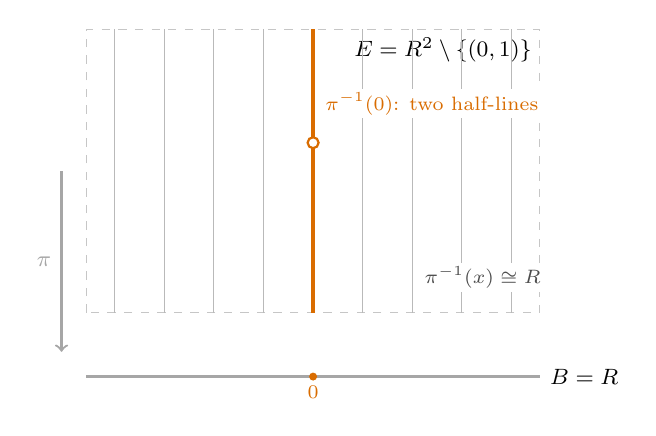
\begin{tikzpicture}[scale=0.9]
\draw[gray!45, dashed] (-3.2,-1.4) rectangle (3.2,2.6); \node[font=\footnotesize, anchor=north east, fill=white, inner sep=1.5pt] at (3.15,2.55) {$E = \mathbb{R}^2 \setminus \{(0,1)\}$};
\draw[gray!55] (-2.80,-1.4) -- (-2.80,2.6);
\draw[gray!55] (-2.10,-1.4) -- (-2.10,2.6);
\draw[gray!55] (-1.40,-1.4) -- (-1.40,2.6);
\draw[gray!55] (-0.70,-1.4) -- (-0.70,2.6);
\draw[gray!55] (0.70,-1.4) -- (0.70,2.6);
\draw[gray!55] (1.40,-1.4) -- (1.40,2.6);
\draw[gray!55] (2.10,-1.4) -- (2.10,2.6);
\draw[gray!55] (2.80,-1.4) -- (2.80,2.6);
\draw[orange!85!black, very thick] (0,-1.4) -- (0,0.93); \draw[orange!85!black, very thick] (0,1.07) -- (0,2.6);
\draw[orange!85!black, fill=white, thick] (0,1) circle (2.2pt);
\node[orange!85!black, font=\scriptsize, anchor=west, align=left, fill=white, inner sep=1.2pt] at (0.12,1.55) {$\pi^{-1}(0)$: two half-lines};
\node[gray!60!black, font=\scriptsize, anchor=west, fill=white, inner sep=1.2pt] at (1.52,-0.9) {$\pi^{-1}(x) \cong \mathbb{R}$};
\draw[->, thick, gray!70] (-3.55,0.6) -- node[left, font=\footnotesize] {$\pi$} (-3.55,-1.95);
\draw[thick, gray!70] (-3.2,-2.3) -- (3.2,-2.3) node[right, font=\footnotesize, text=black] {$B = \mathbb{R}$};
\fill[orange!85!black] (0,-2.3) circle (1.6pt) node[below, font=\scriptsize] {$0$};
\end{tikzpicture}
